\section{Anwendungsschicht}
	Netzwerkanwendung: \newline
	\begin{itemize}
  	\item Anwendungsprozesse auf verschiedenen Hosts
  	\item kann direkt unter Verwendung der Dienste der Transportschicht implementiert werden
	  \item standardisieret Anwendung benutzen ein Anwendungsprotokoll, das das Format der Nachrichten und das Verhalten beim Empfang festlegt
	\end{itemize}
	\subsection{Paradigmen}
		\subsubsection{Client-Server}
			Server stellt Dienst zur Verfügung, der vom Client angefragt wird
		\subsubsection{Wechselnde Rollen}
			Hosts übernehmen mal die eine, mal die andere Rolle
		\subsubsection{Verteilte Anwendung}
			Besteht aus mehreren unabhängigen Anwendungen, die zusammen wie eine einzelne Anwendung erscheinen (z.B. WebShop mit Web-Server, Applikations-Server und Datenbank), Koordination ist zwar verteilt, findet aber für das Gesamtsystem statt
		\subsubsection{Peer-to-Peer}
			Vernetzung von Gleichen: \newline
			\begin{itemize}
				\item dezentrale Architektur (z.B. Bitcoin)
				\item Hybridarchitektur: Initialisierung findet über zentrale Architektur statt, Anwendung dezentral zwischen Hosts
			\end{itemize}
		\subsubsection{Anforderungen}
			\begin{itemize}
				\item Verlust
				\item Bitrate
				\item Verzögerungszeit
			\end{itemize}
	\subsection{Hypertext Transfere Protocol (HTTP)}
		\subsubsection{Ablauf}
			\begin{enumerate}
				\item Benutzer gibt URI (Uniform Resource Identifier) in Web-Browser ein
				\item URI enthält Host-Namen eines Web-Servers und den Pfad zu einem Objekt
				\item Web-Browser stellt Anfrage an Web-Server für dieses Objekt
				\item Web-Server liefert Objekt an Web-Browser zurück
				\item Web-Browser stellt Objekt für Nutzer lesbar da
			\end{enumerate}
		\subsubsection{Format der Anfragen}
			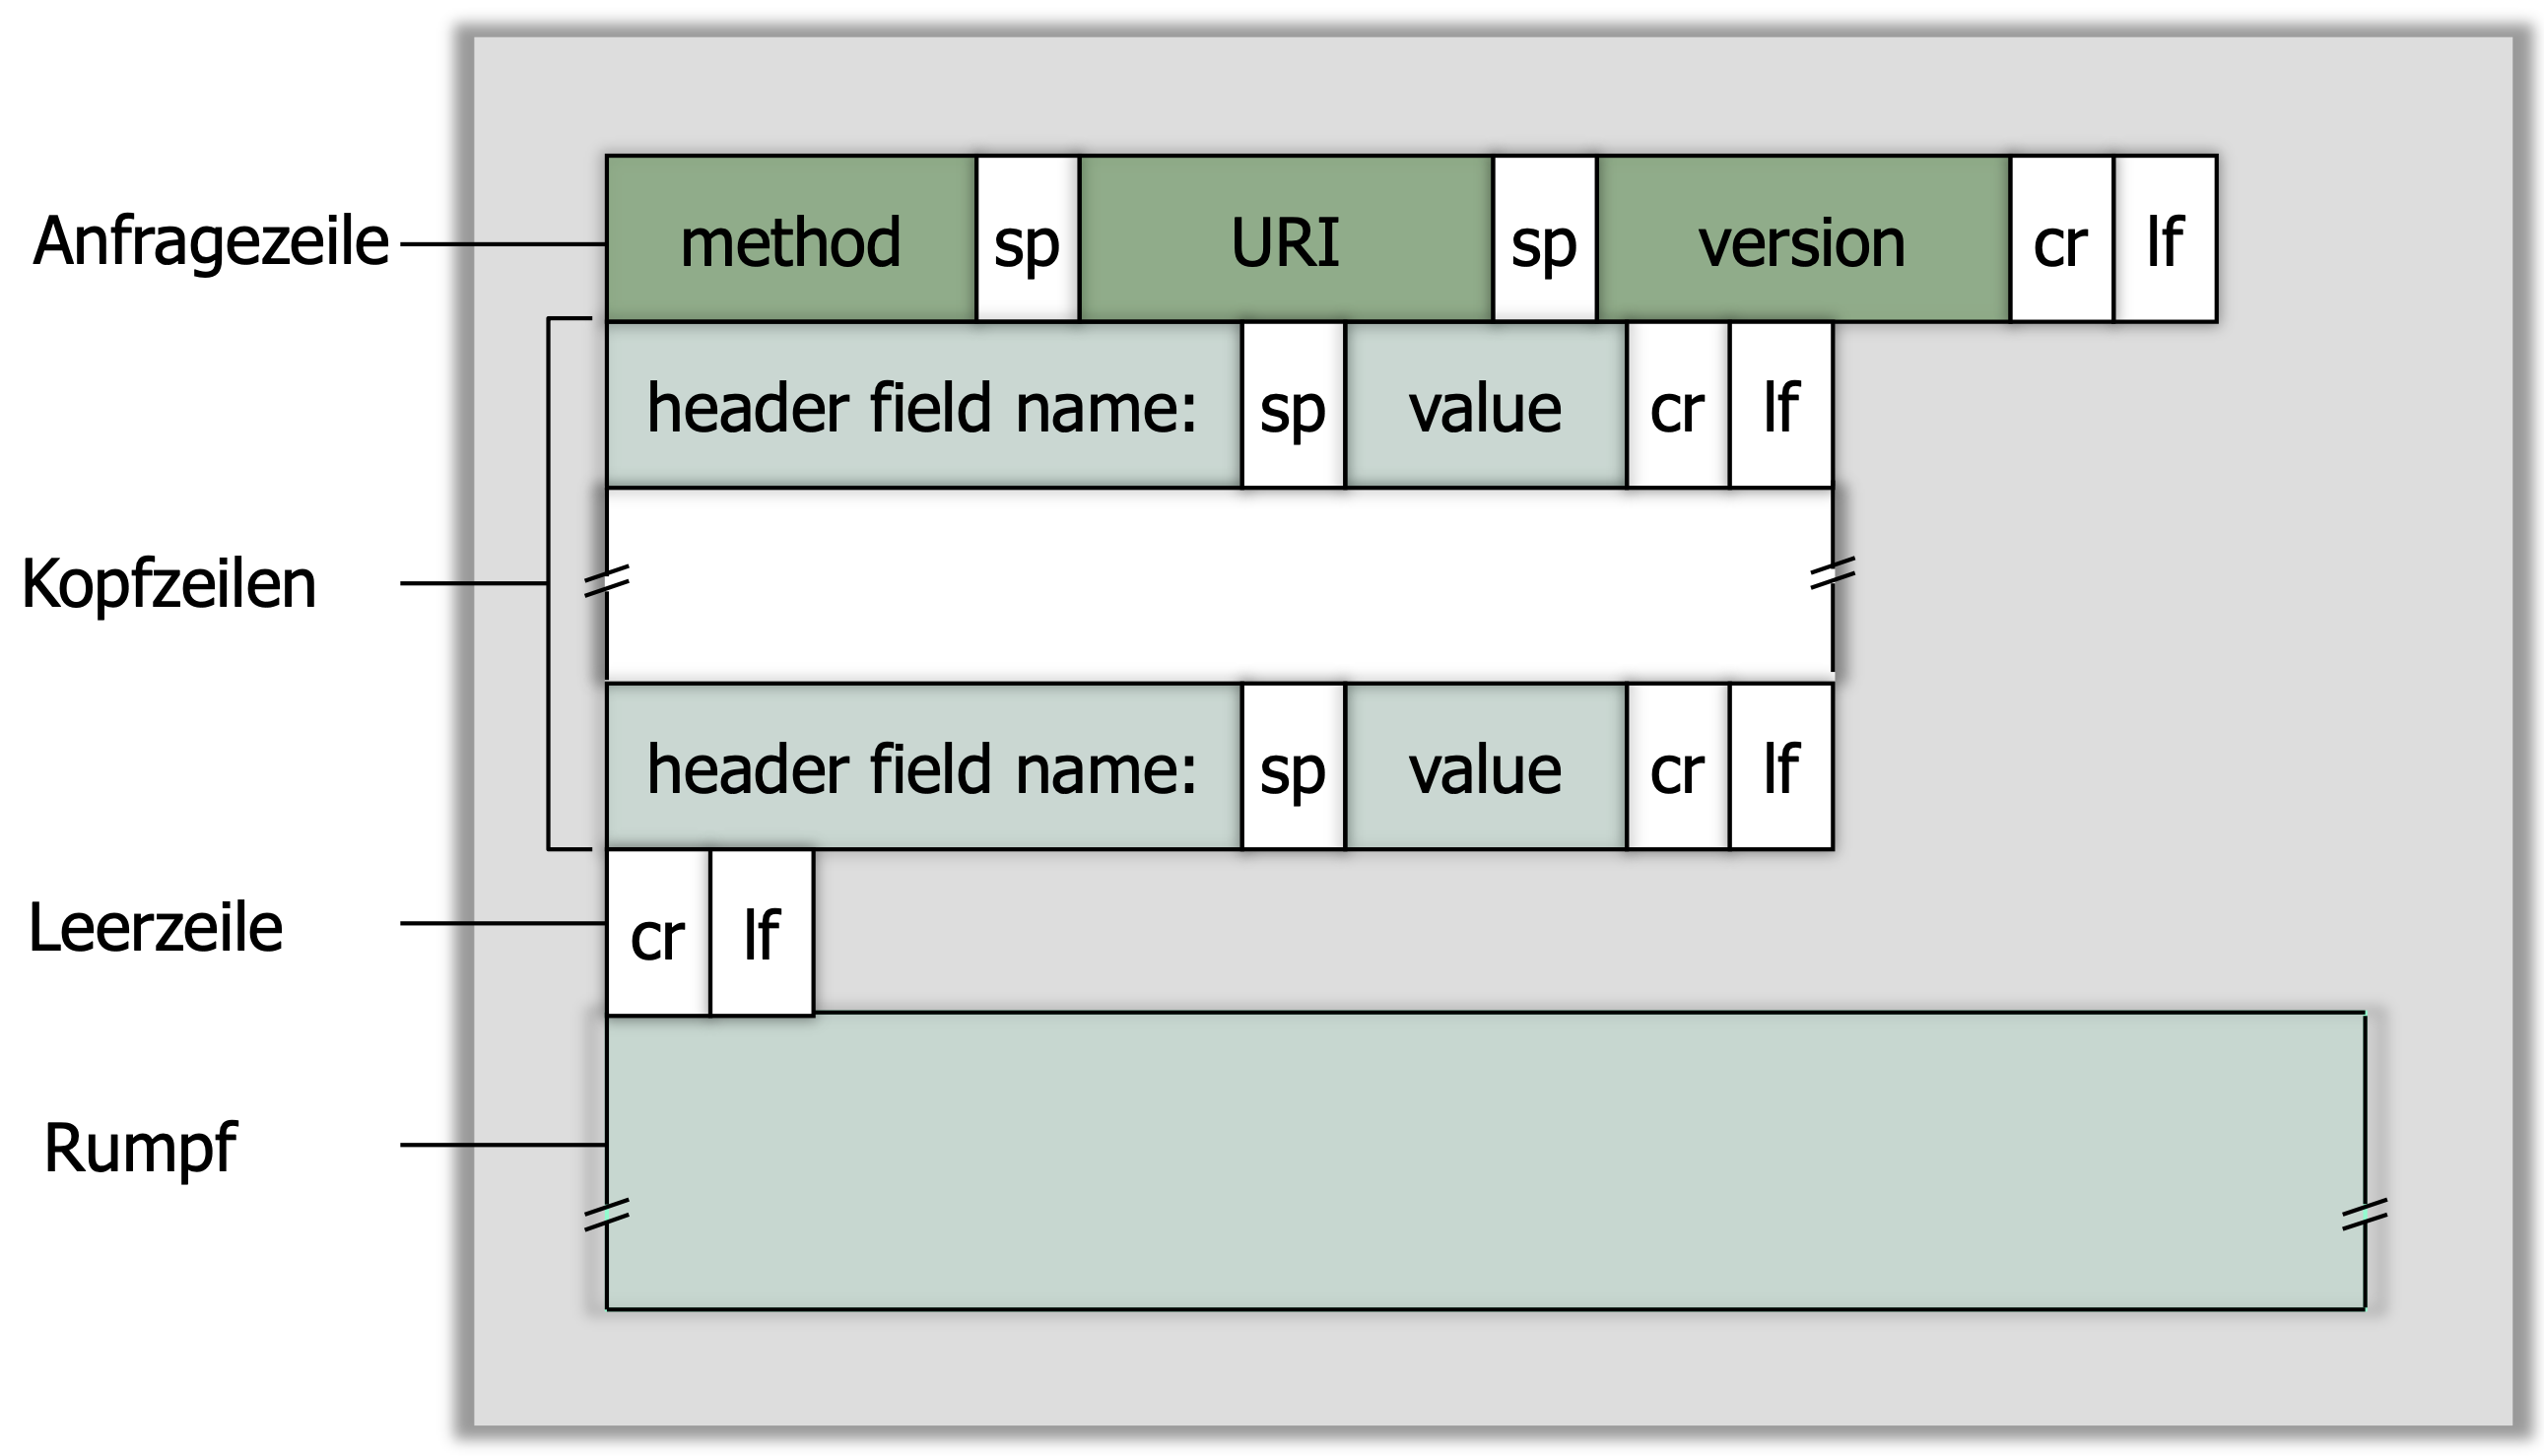
\includegraphics[scale=0.25]{Anfragenachricht_HTTP.png}
		\subsubsection{Anfragenachricht}
			\begin{itemize}
				\item Methoden: 
					\begin{itemize}
						\item GET: Abruf eines Dokuments, besteht aus Methode, URI, Version
						\item HEAD: Abruf von Metainformationen eines Dokuments
						\item POST: Übergabe von Informationen an Server
						\item PUT
						\item DELET
					\end{itemize}
				\item Kopfzeilen:
					\begin{itemize}
						\item Typ/Wert-Paare, Typen: Host, User-agent, ...
					\end{itemize}
				\item Rumpf:
					\begin{itemize}
						\item leer bei GET, kann bei POST Inhalt haben
					\end{itemize}
			\end{itemize}
			\begin{center}
				\begin{tabular}{|cc|}
					\hline
					GET: & /somedir/page.html HTTP/1.1 \\
					HOST: & www.someschool.edu \\
					User-agent: & Mozilla/4.0 \\
					Connection: & close \\
					Accept-language: & de-de \\
					\hline
				\end{tabular}
			\end{center}
		\subsubsection{Format der Antworten}
			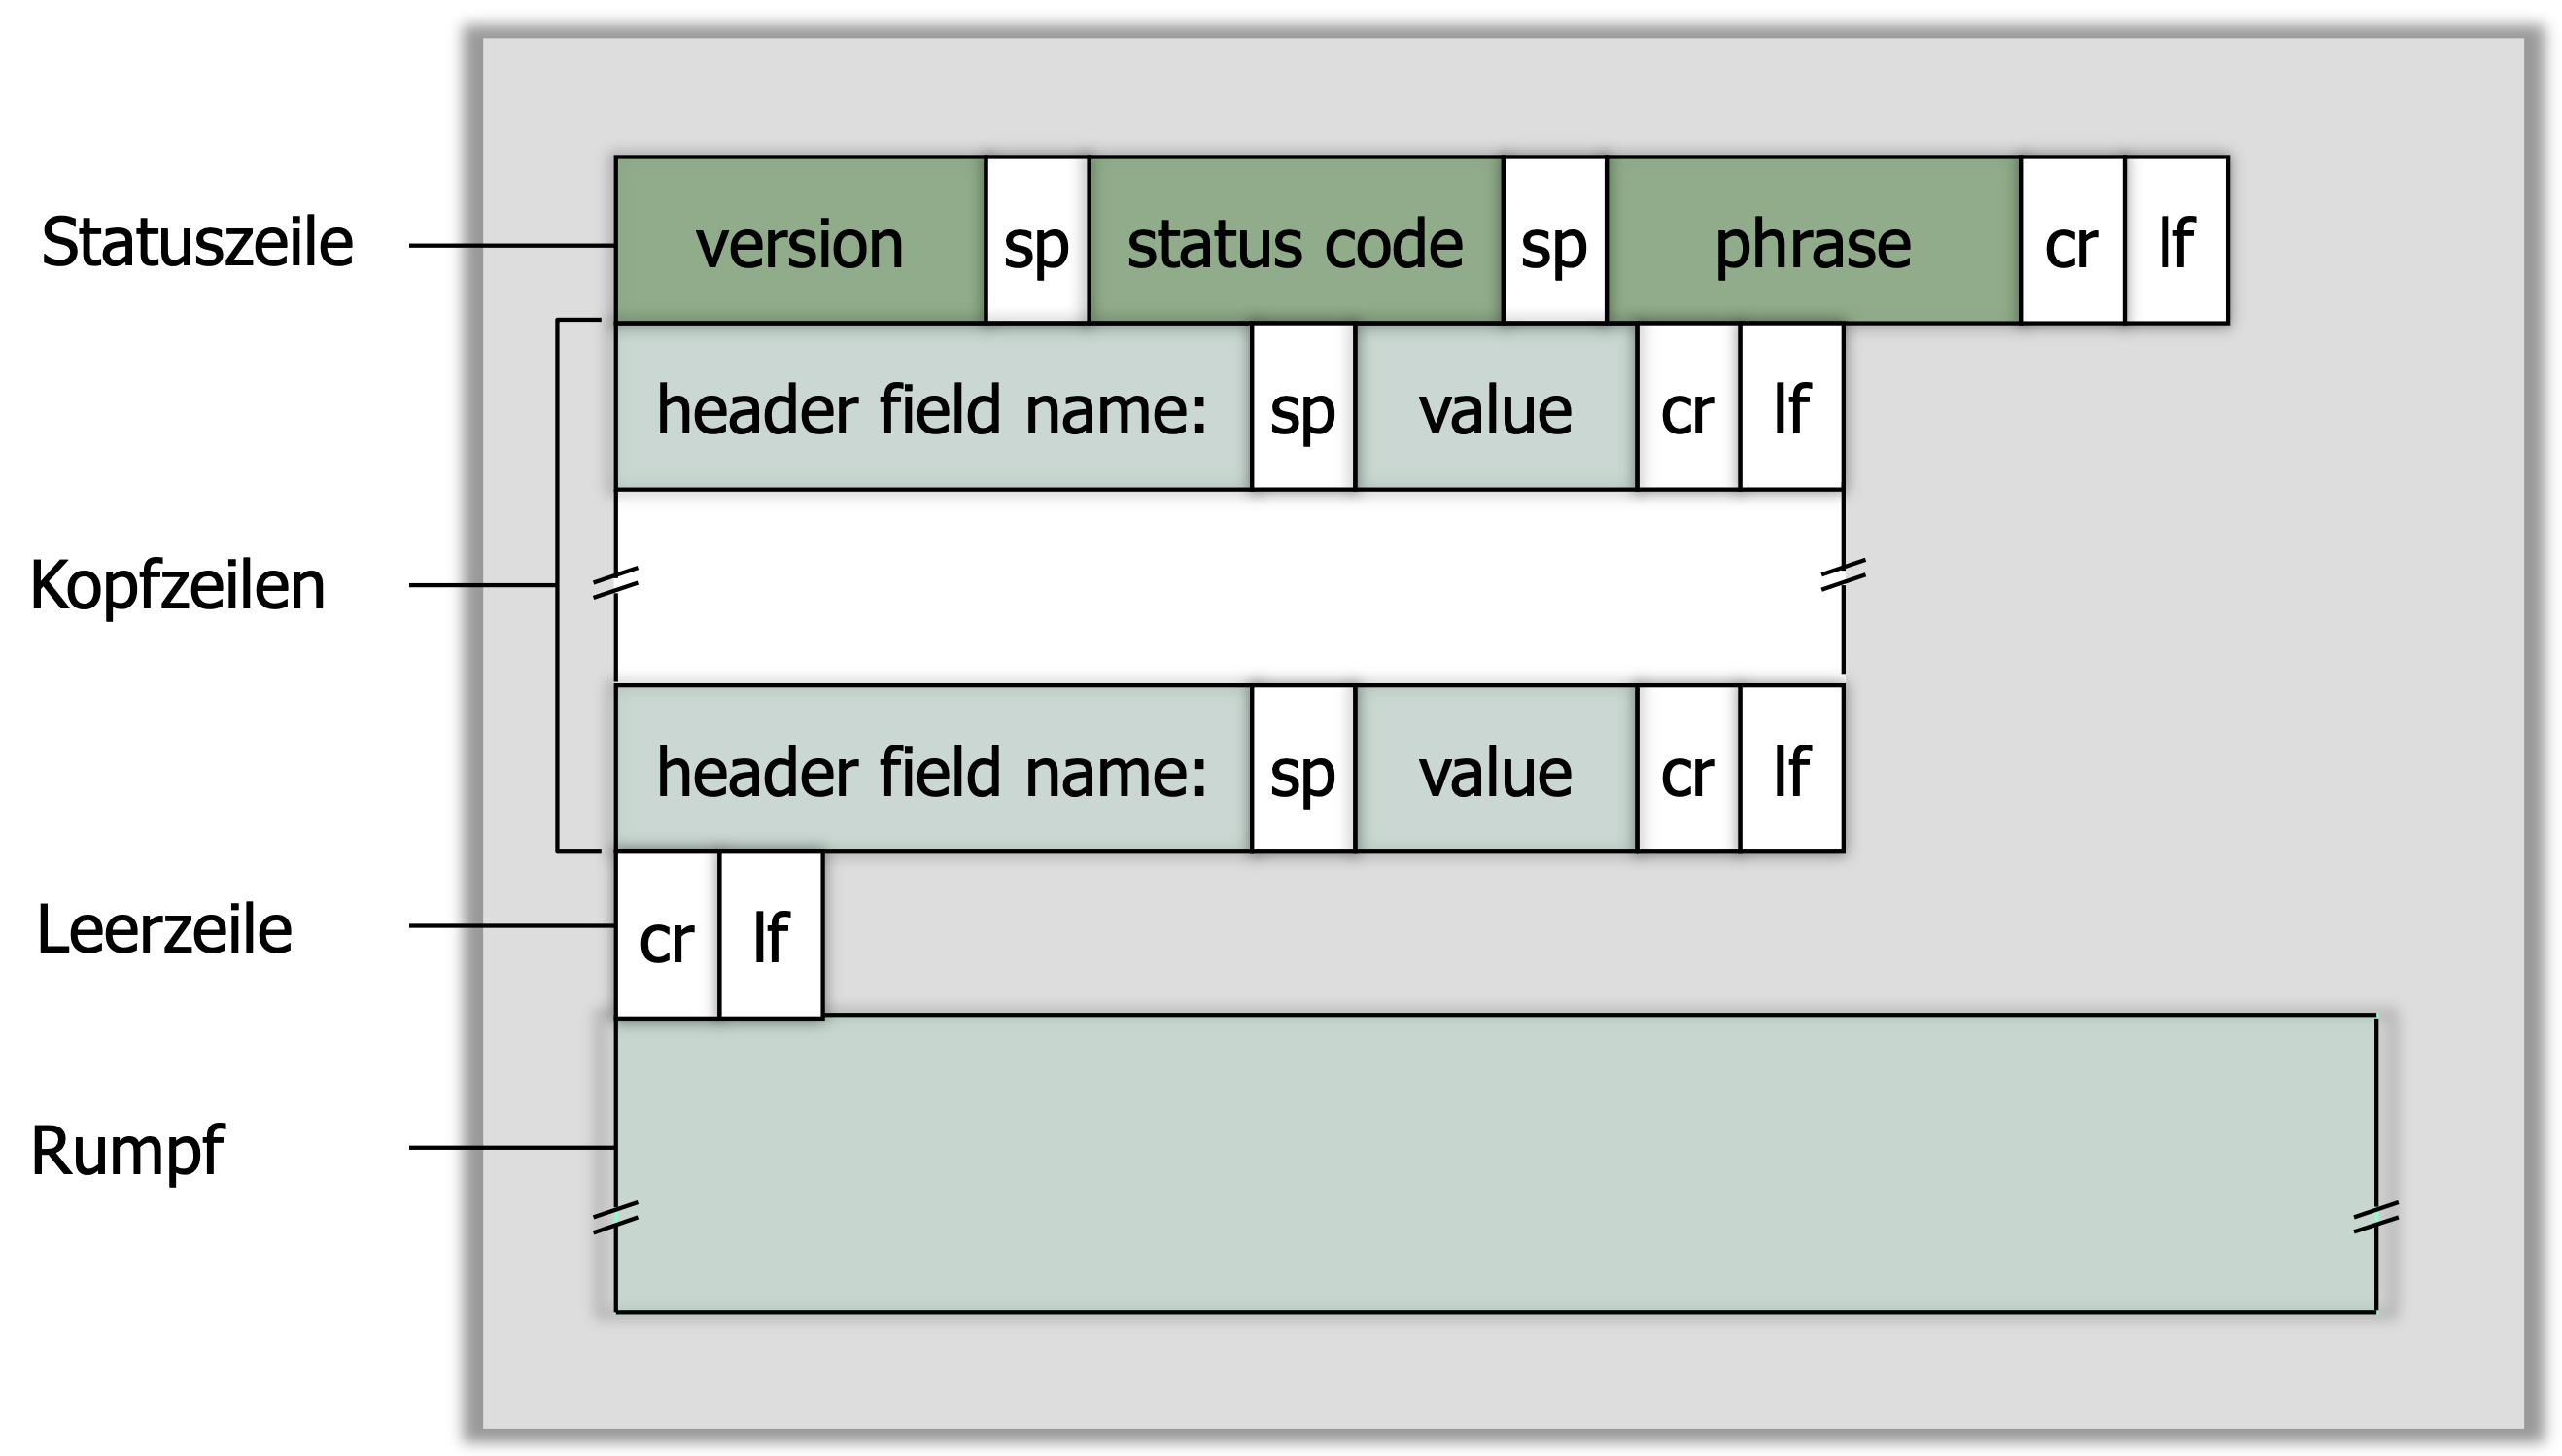
\includegraphics[scale=0.25]{Antwortnachricht_HTTP.png}
		\subsubsection{Antwortnachricht}
			\begin{center}
				\begin{tabular}{|cc|}
					\hline
					HTTP/1.1 & 200 OK \\
					Connection: & close \\
					Date: & Thu, 06 Aug 1998 12:00:15 GMT \\
					Server: & Apache/1.3.0 (Unix) \\
					Last-Modified: & Mon, 22 Jun 1998 ... \\
					Content-Length: & 6821 \\
					Content-Type: & text/html \\
					& \\
					data & data \\
					\hline
				\end{tabular}
			\end{center}
		\subsubsection{HTTP-Ablauf}
			\textbf{Nicht-persistentes HTTP}: \newline
				Für jedes Objekt wird eine einzelne TCP-Verbindung aufgebaut. Entweder Basisseite und eingebettete Objekte sequentiell oder parallele Verbindung für eingebettete Objekte
				\newline \newline
			\textbf{Persistentes HTTP}: \newline
				Server lässt Verbindung bestehen, alle Objekte werden über eine TCP Verbindung gesendet. Ohne Pipelining wird jedes Objekt einzeln Angefragt, mit alle auf einmal
			
		\subsubsection{Antwortzeit}
			Basisseite: Aufbau der TCP-Verbindung (1x RTT) + Anfrage hin und Antwort zurück (1x RTT) $\Rarr$ 2RTT + Zeit zum Senden + weitere Wartezeiten durch TCP \newline
			\begin{center}
				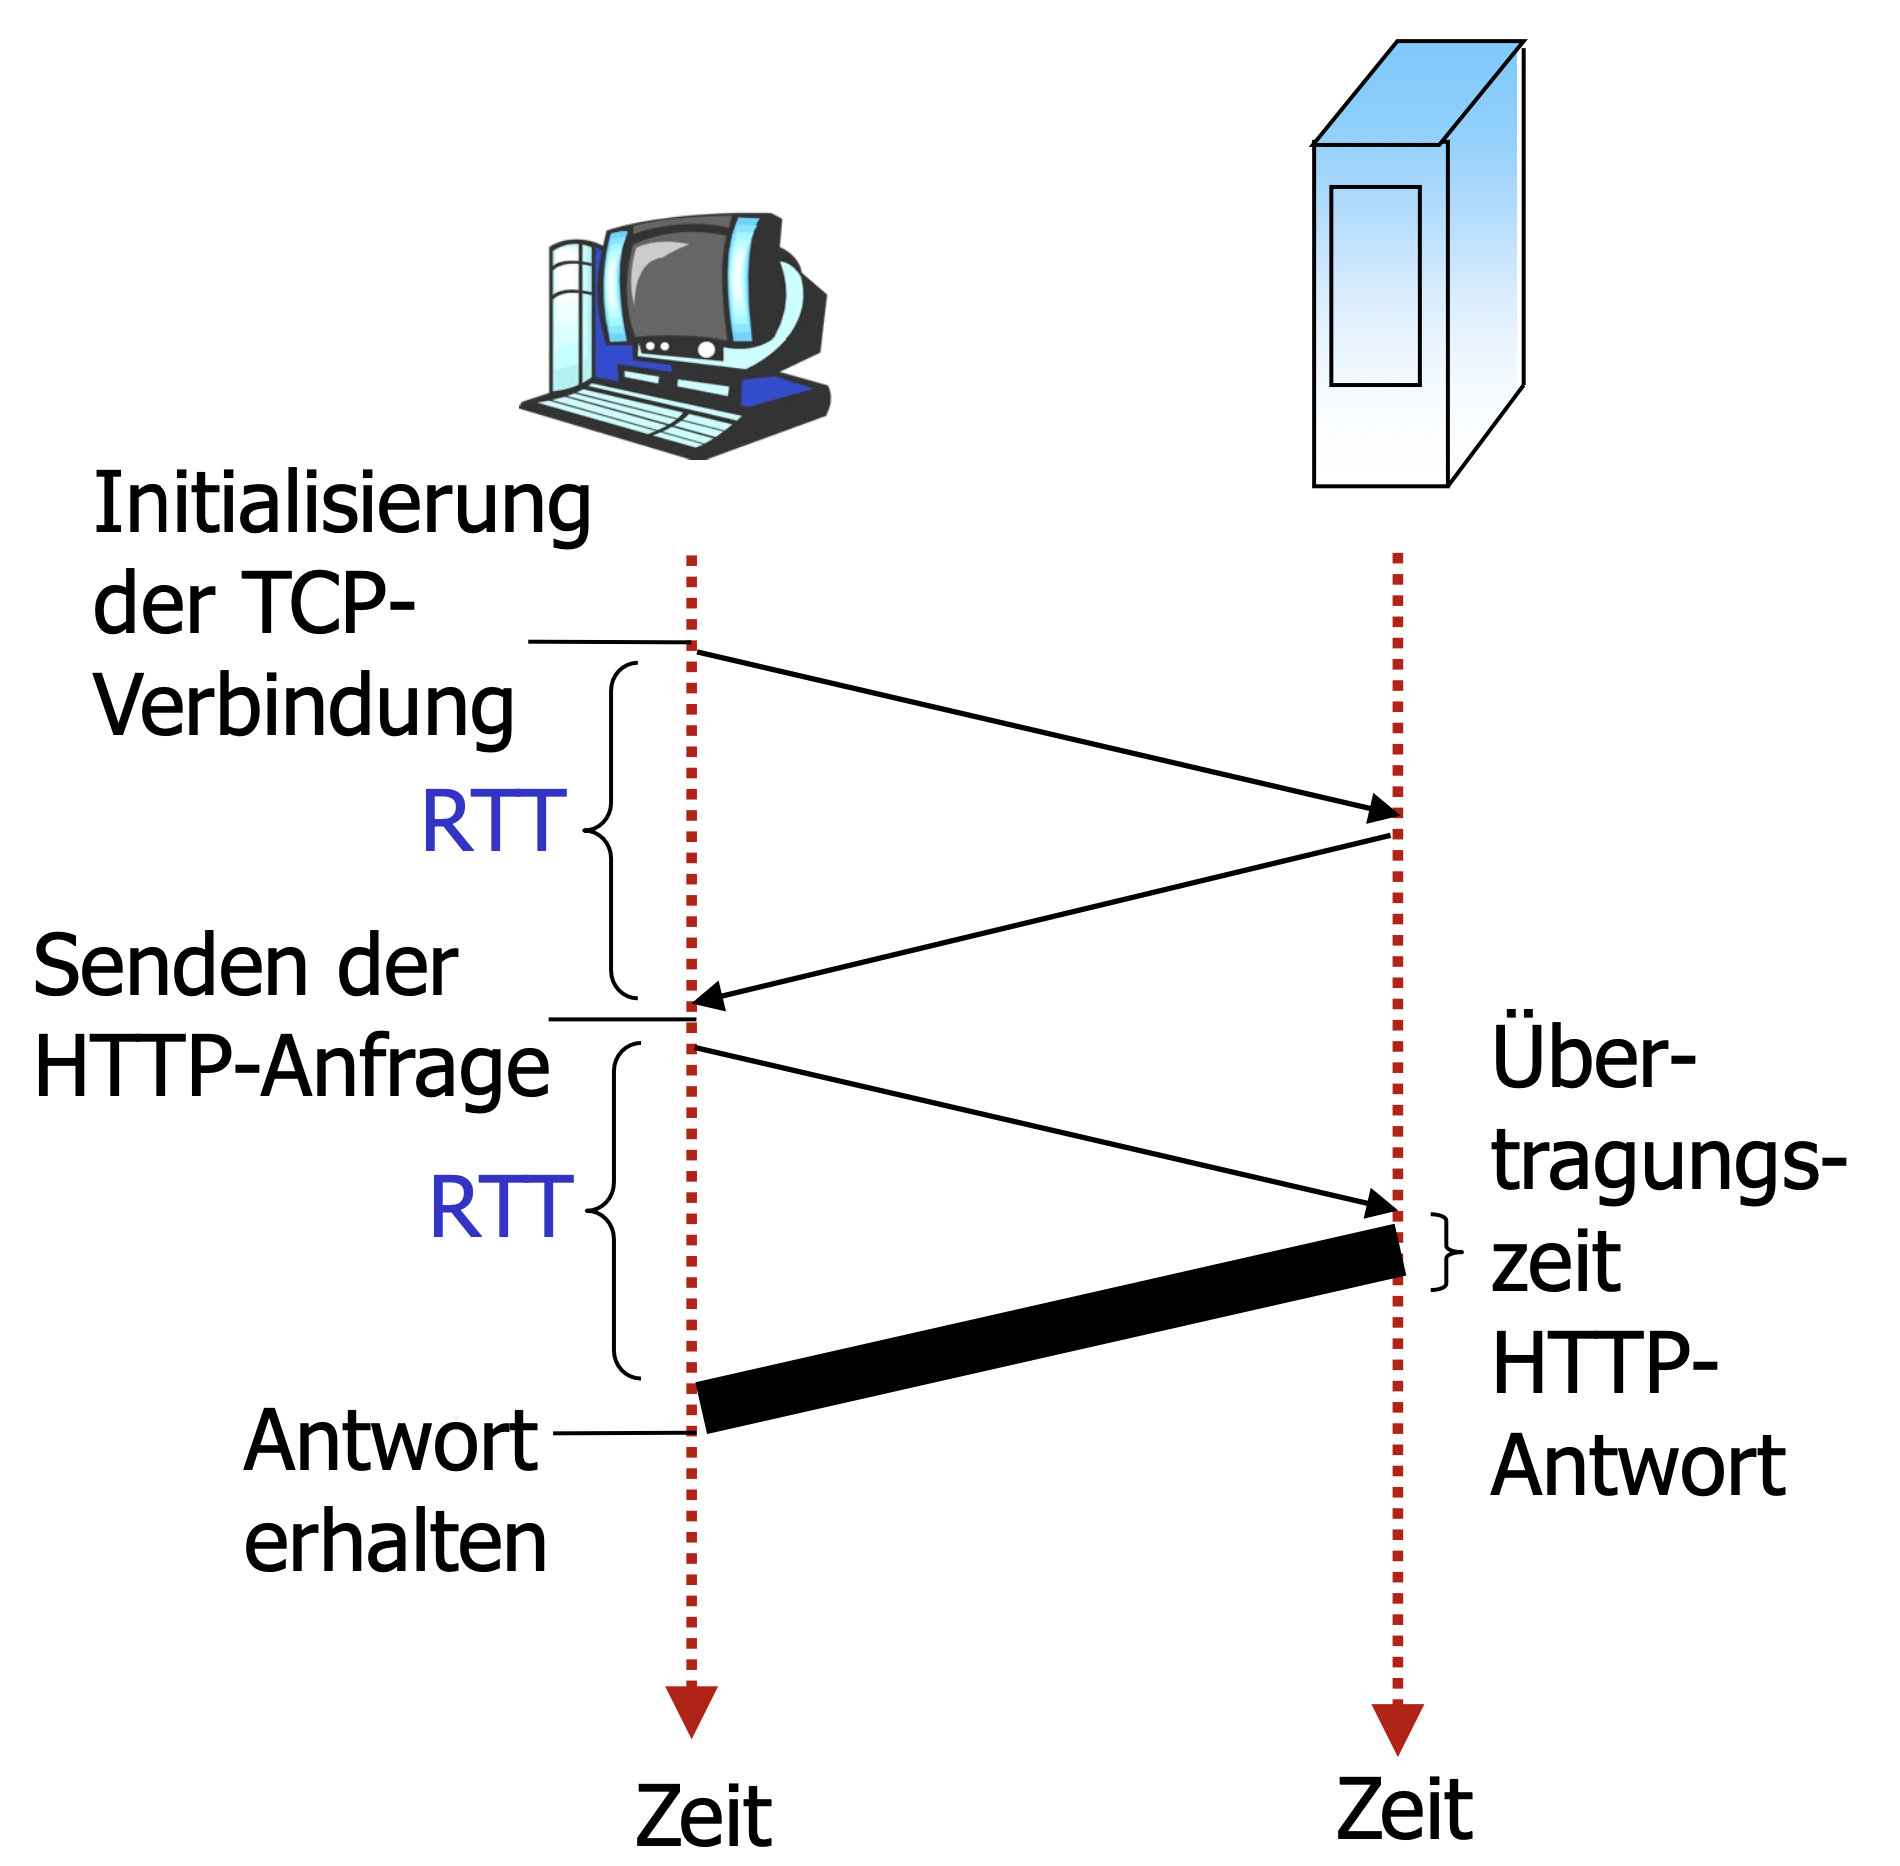
\includegraphics[scale=0.25]{Antwortzeit_HTTP_Basis.png}	
			\end{center}
		\subsubsection{Dynamische Inhalte}
			\textbf{Common Gate Interface (CGI)} verarbeitet als externer Prozess die Information und liefert neue HTML-Seite an Server \newline \newline
			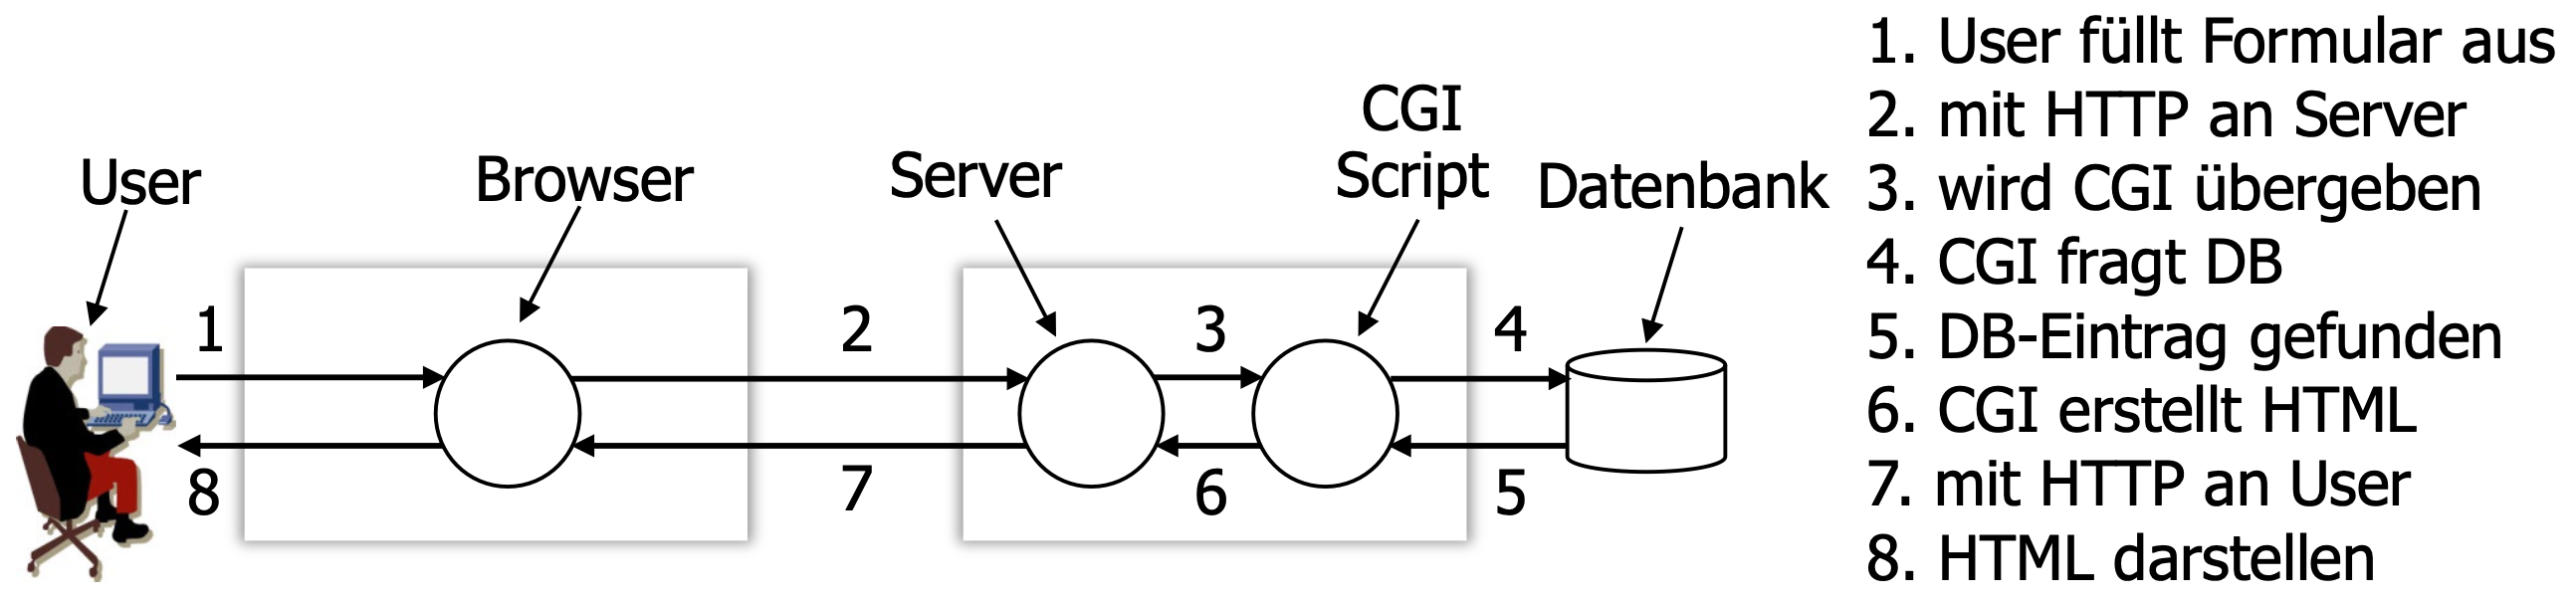
\includegraphics[scale=0.25]{CGI_HTML.png}
			\newline
			\textbf{Scripting:} Durch Interpretation von eingebetteten Skripten können dynamische Inhalte erzeugt werden.\newline \newline
			Serverseitig: im HTML ist Code eingebettet, der vom Server interpretiert wird und dabei HTML erzeugt, z.B. PHP \newline \newline
			Clientseitig: im HTML ist Code eingebettet, der vom Client interpretiert wird, z.B. JavaScript
		\subsubsection{Caching}
			Cache (Proxy Server) ist Server für Web-Browser und Client für Web-Server, der als Zwischenspeicher zur Verringerung der Wartezeit des Nutzers und des Netzverkehrs dient
			\begin{center}
				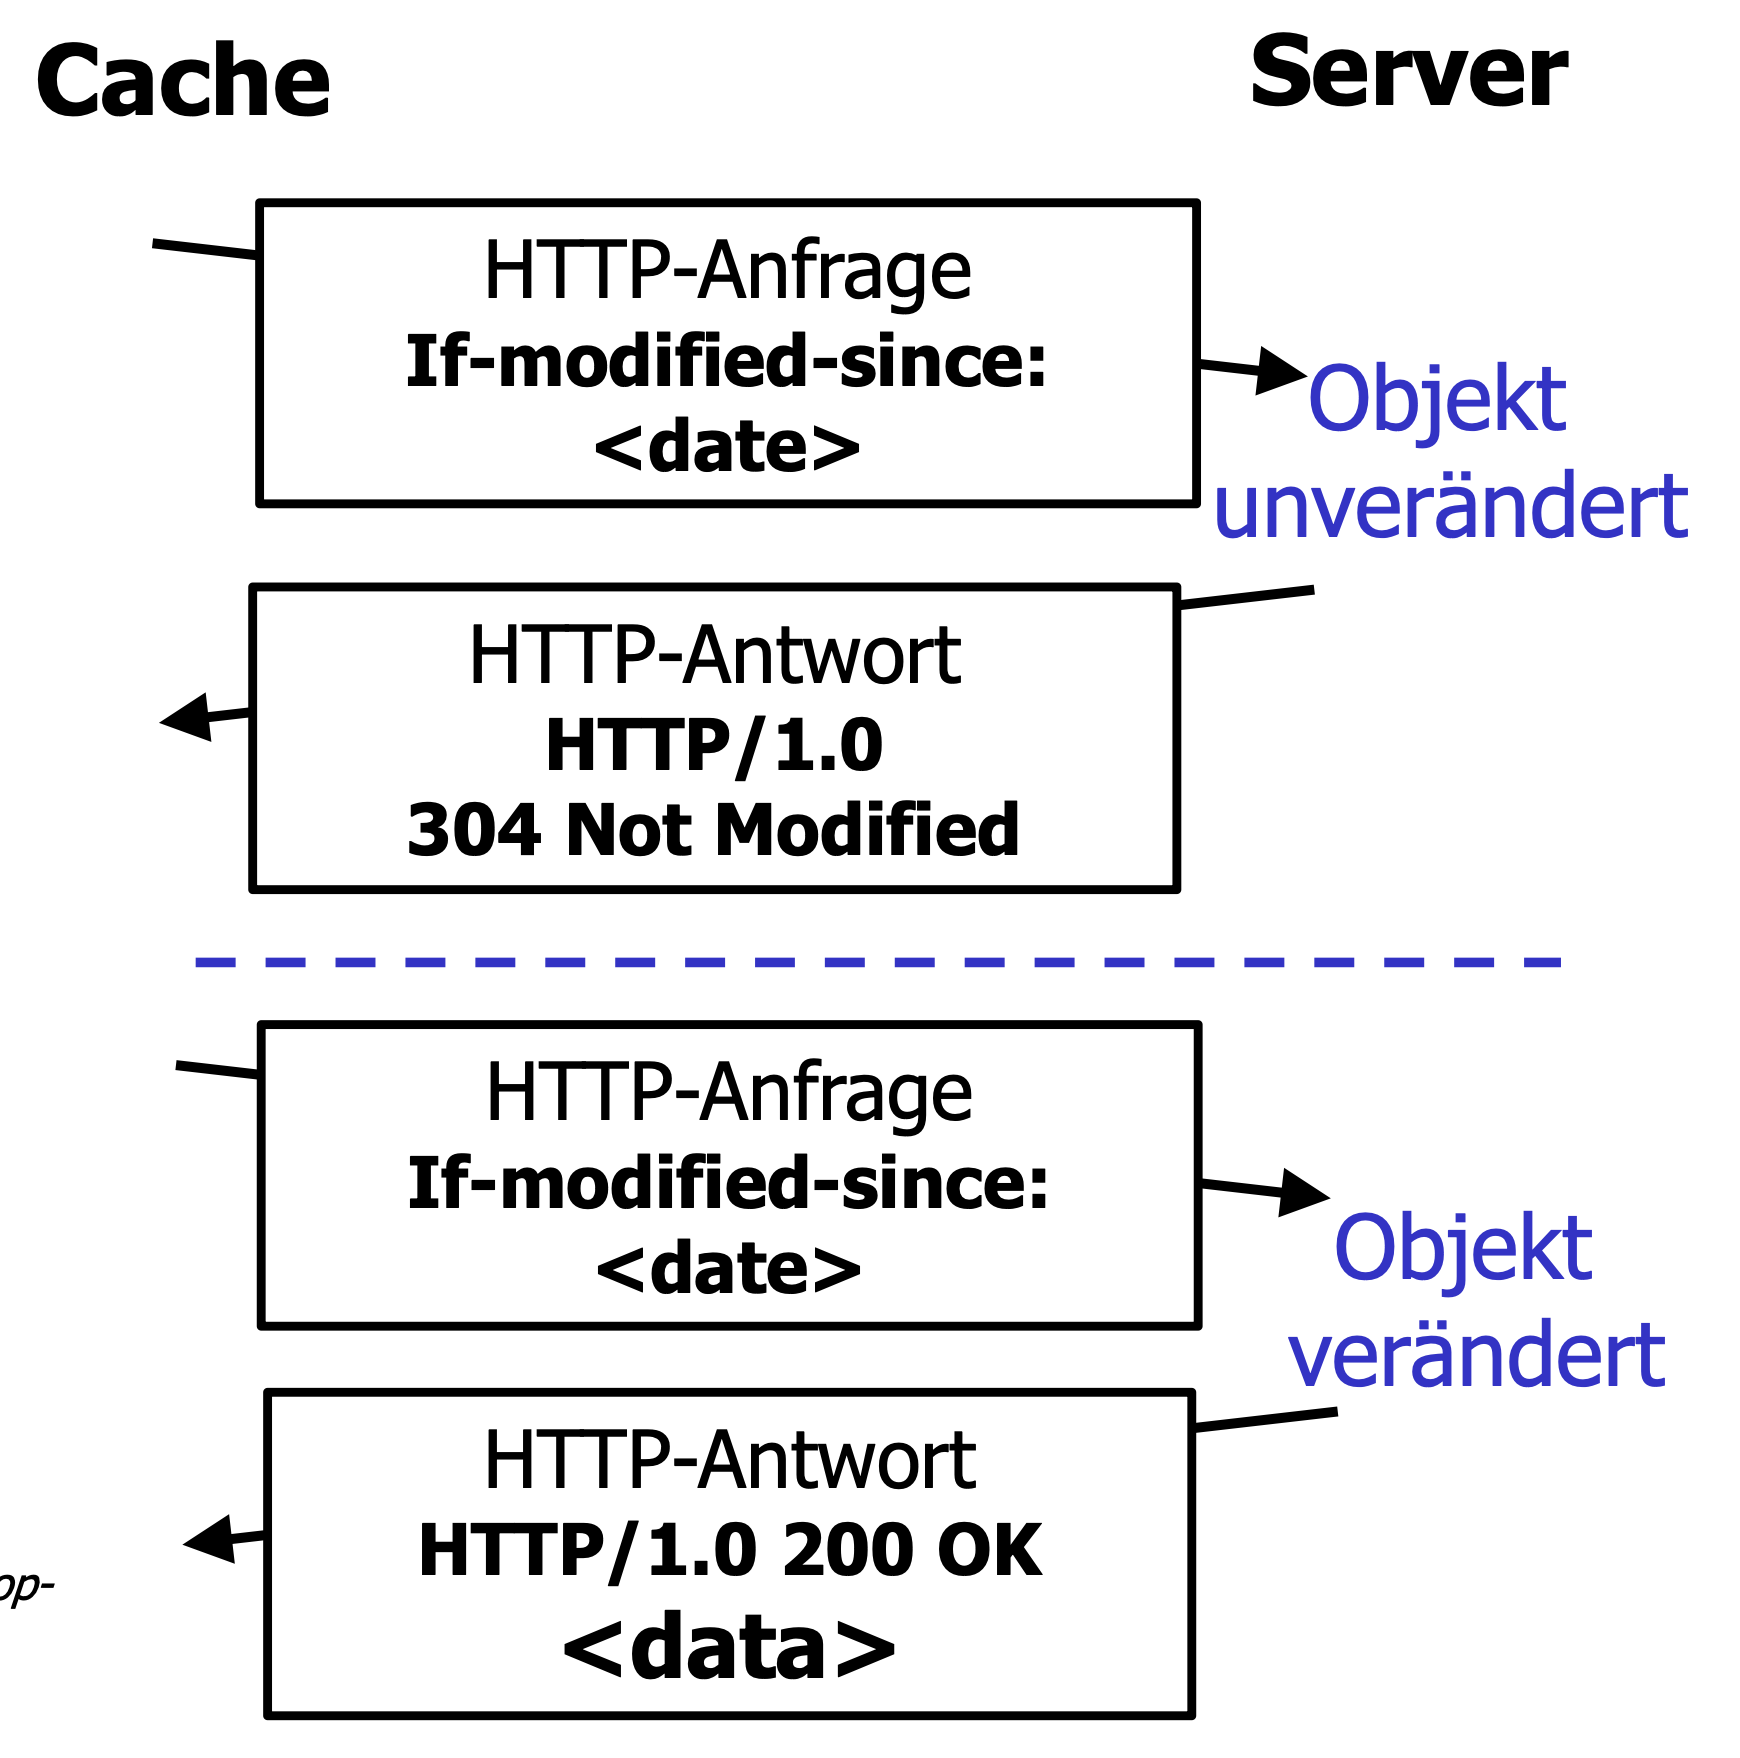
\includegraphics[scale=0.25]{Cache_Server_HTML.png}
			\end{center}
		\subsubsection{HTTP/2}
			Wesentliche Elemente: 
			\begin{itemize}
				\item gleiche Methoden
				\item binäres statt textbasiertes Format
				\item Multiplexing verschiedener Ströme über eine TCP-Verbindung, Vermeidung von Head-of-Line (HOL) Blockierung durch große Objekte durch Aufteilung in kleinere Frames und Interleaving
				\item Header-Kompression
				\item Server-Push
			\end{itemize}
	\subsection{File Transfere Protocol (FTP)}
		\begin{itemize}
			\item Übertragung zwischen zwei Hosts
			\item eine TCP-Verbindung (Port 21) zur Steuerung
			\item lesbare Kommandos: USER username, PASS password, LIST, PETR filename, STOR filename, ...
			\item jeweils eine TCP-Verbindung (Port 20) zur  Übertragung einer Datei
			\item 'out-of-band-controll'
		\end{itemize}
		\begin{center}
			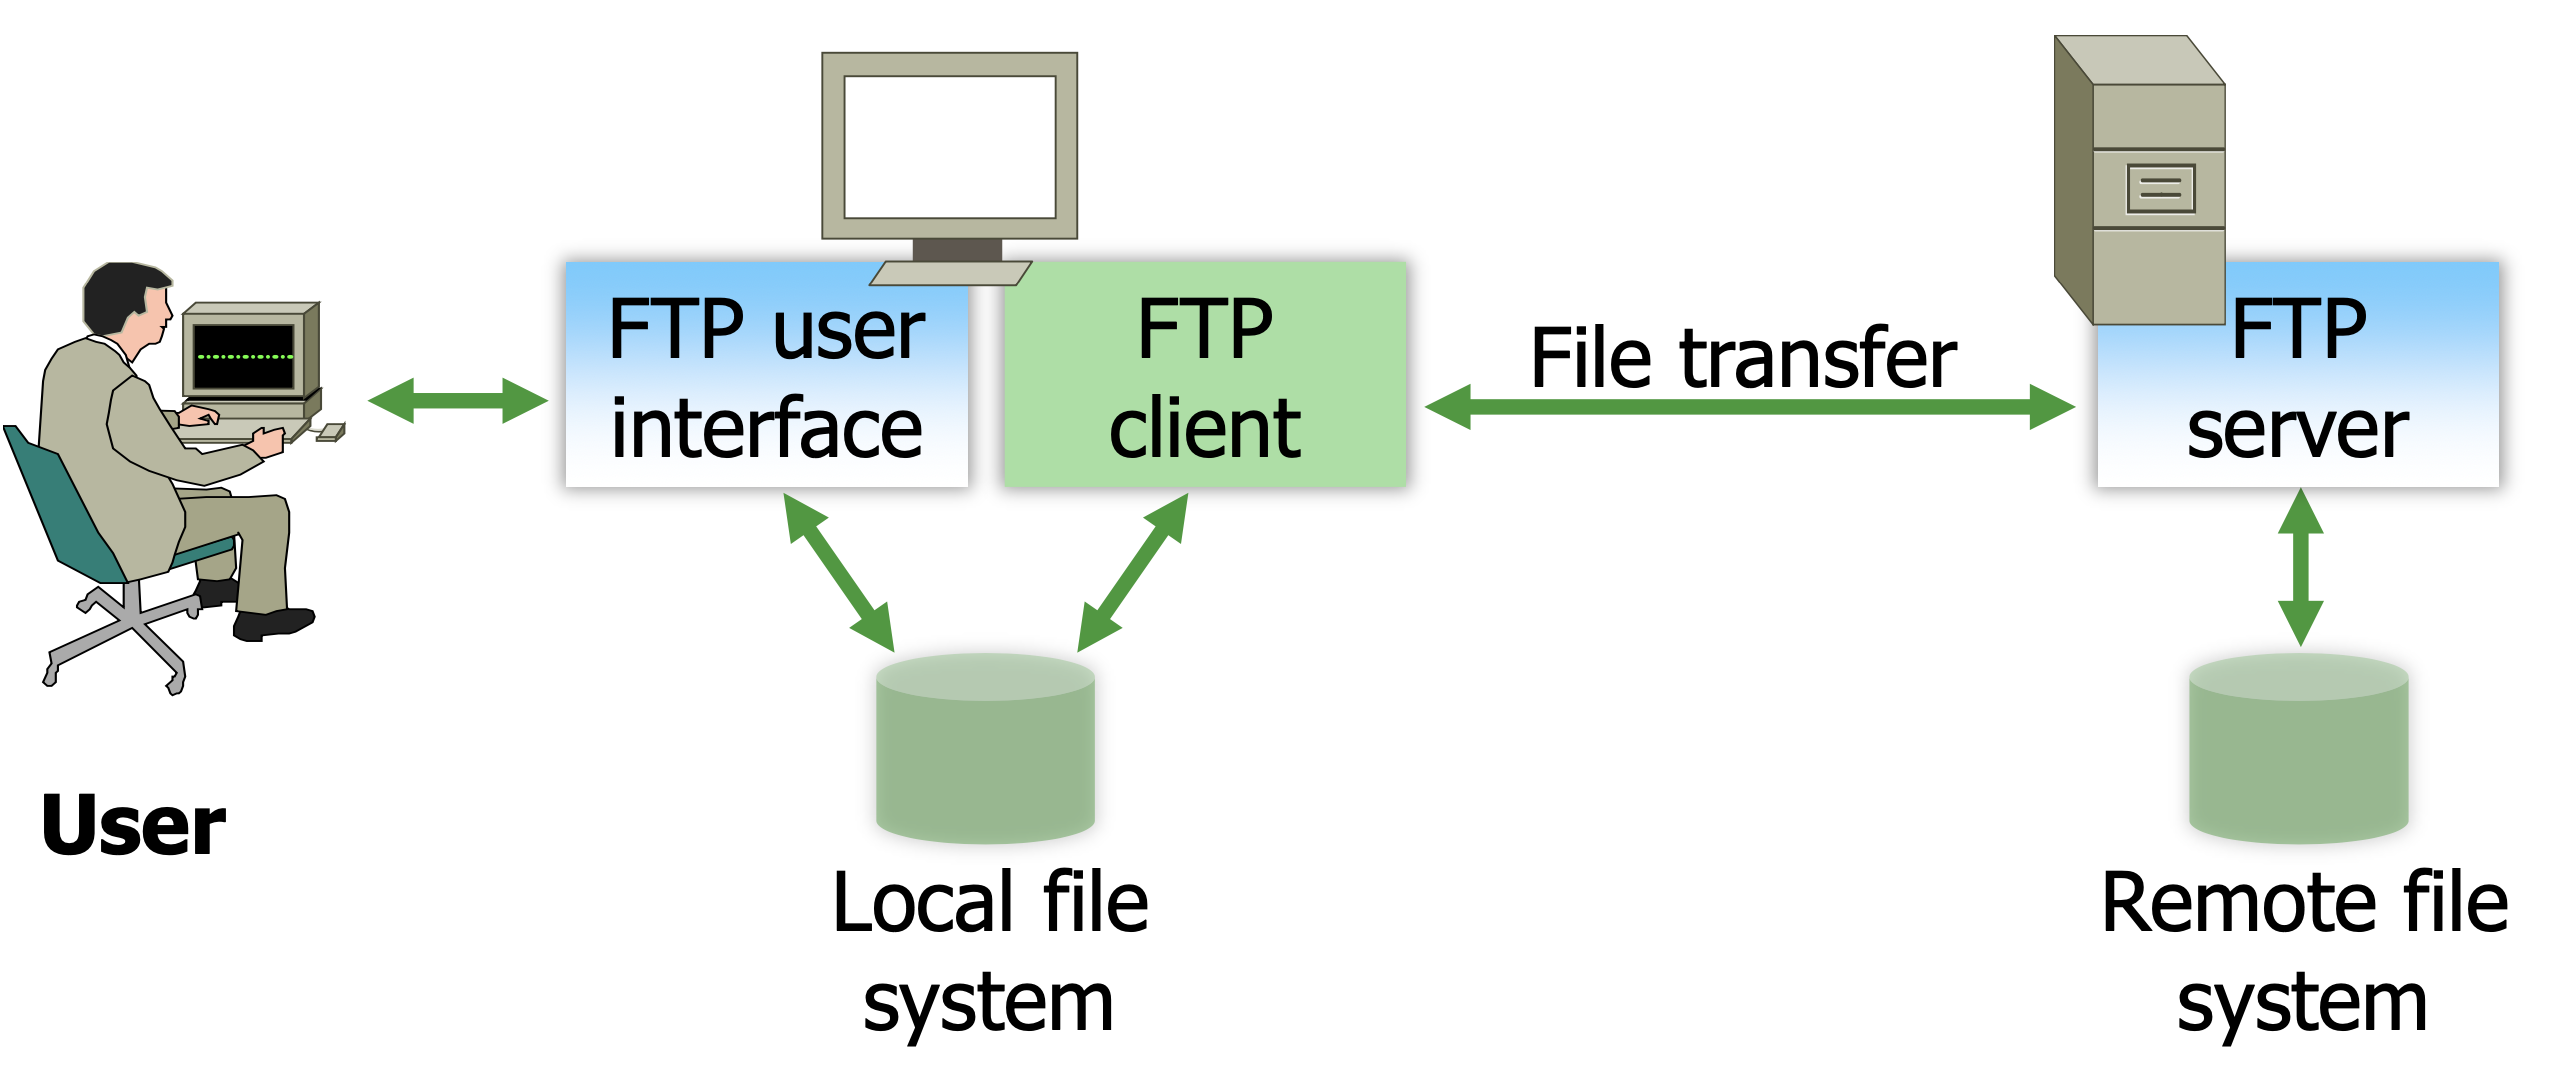
\includegraphics[scale=0.25]{FTP.png}
		\end{center}
	\subsection{Simple Mail Transfer Protocol (SMTP)}
		\begin{itemize}
			\item Nachrichten im ASCII-Format, Kopf, Rumpf
			\item andere Daten werden in ASCII umgewandelt angehängt
			\item Versenden mit SMPT über TCP (lesbar)
			\item Abholen mit POP3, IMAP, HTTP (lesbar)
		\end{itemize}
		\begin{center}
			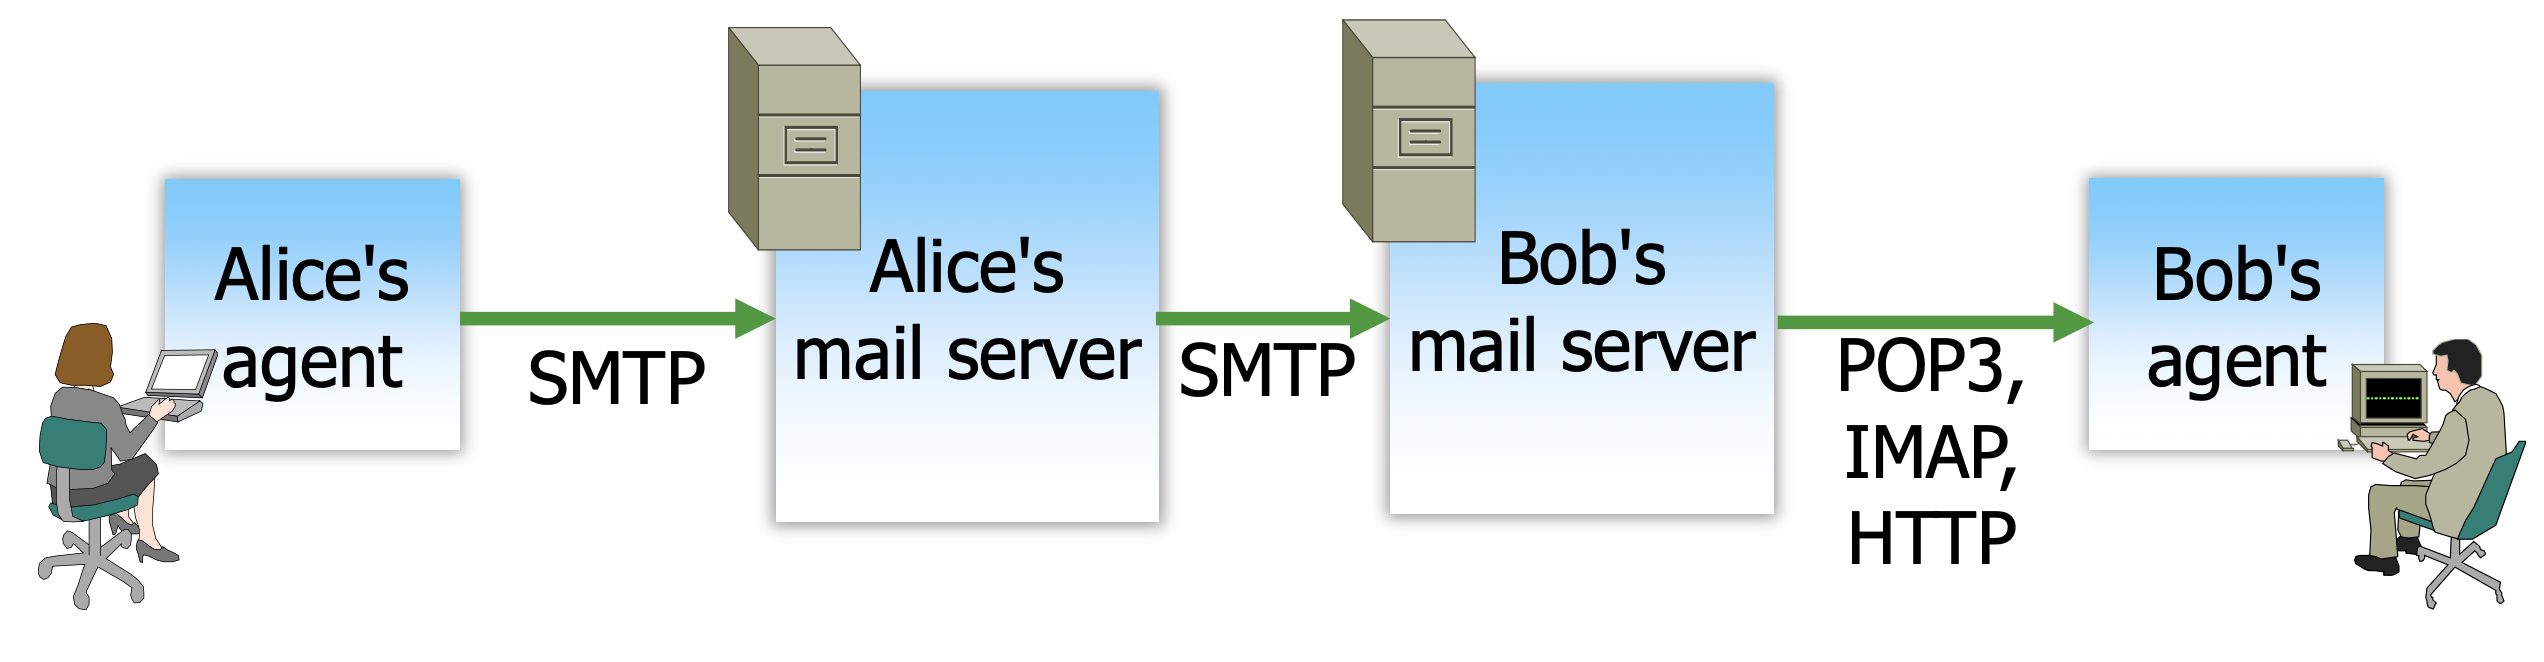
\includegraphics[scale=0.25]{SMTP.png}
		\end{center}
		\begin{itemize}
			\item nutzt TCP (Port 25)
			\item direkte Übertragung: vom Sendenden zu empfangendem Server
			\item drei Phasen der Übertragung:
				\begin{itemize}
					\item Handshake
					\item Nachrichtenübertragung
					\item Abschlussphase
				\end{itemize}
			\item Interaktion mittels Befehlen und Antworten
				\begin{itemize}
					\item Befehle: ASCII-text
					\item Antworten: Statuscode und Text
				\end{itemize}
			\item Nachrichten müssen 7-bit ASCII-text sein
		\end{itemize}
		\subsubsection{Vertraulichkeit und Datenintegrität}
			\begin{enumerate}
				\item Erzeugung eines Hashwerts der E-Mail
				\item Signierung mit privatem Schlüssel $K_A^-$ von Alice
				\item Verschlüsselung der Mail und der Signatur mit $K_S$
				\item Asymmetrische Verschlüsselung von $K_S$ mit dem öffentlichen Schlüssel $K_B^+$ von Bob
			\end{enumerate}
			\begin{center}
				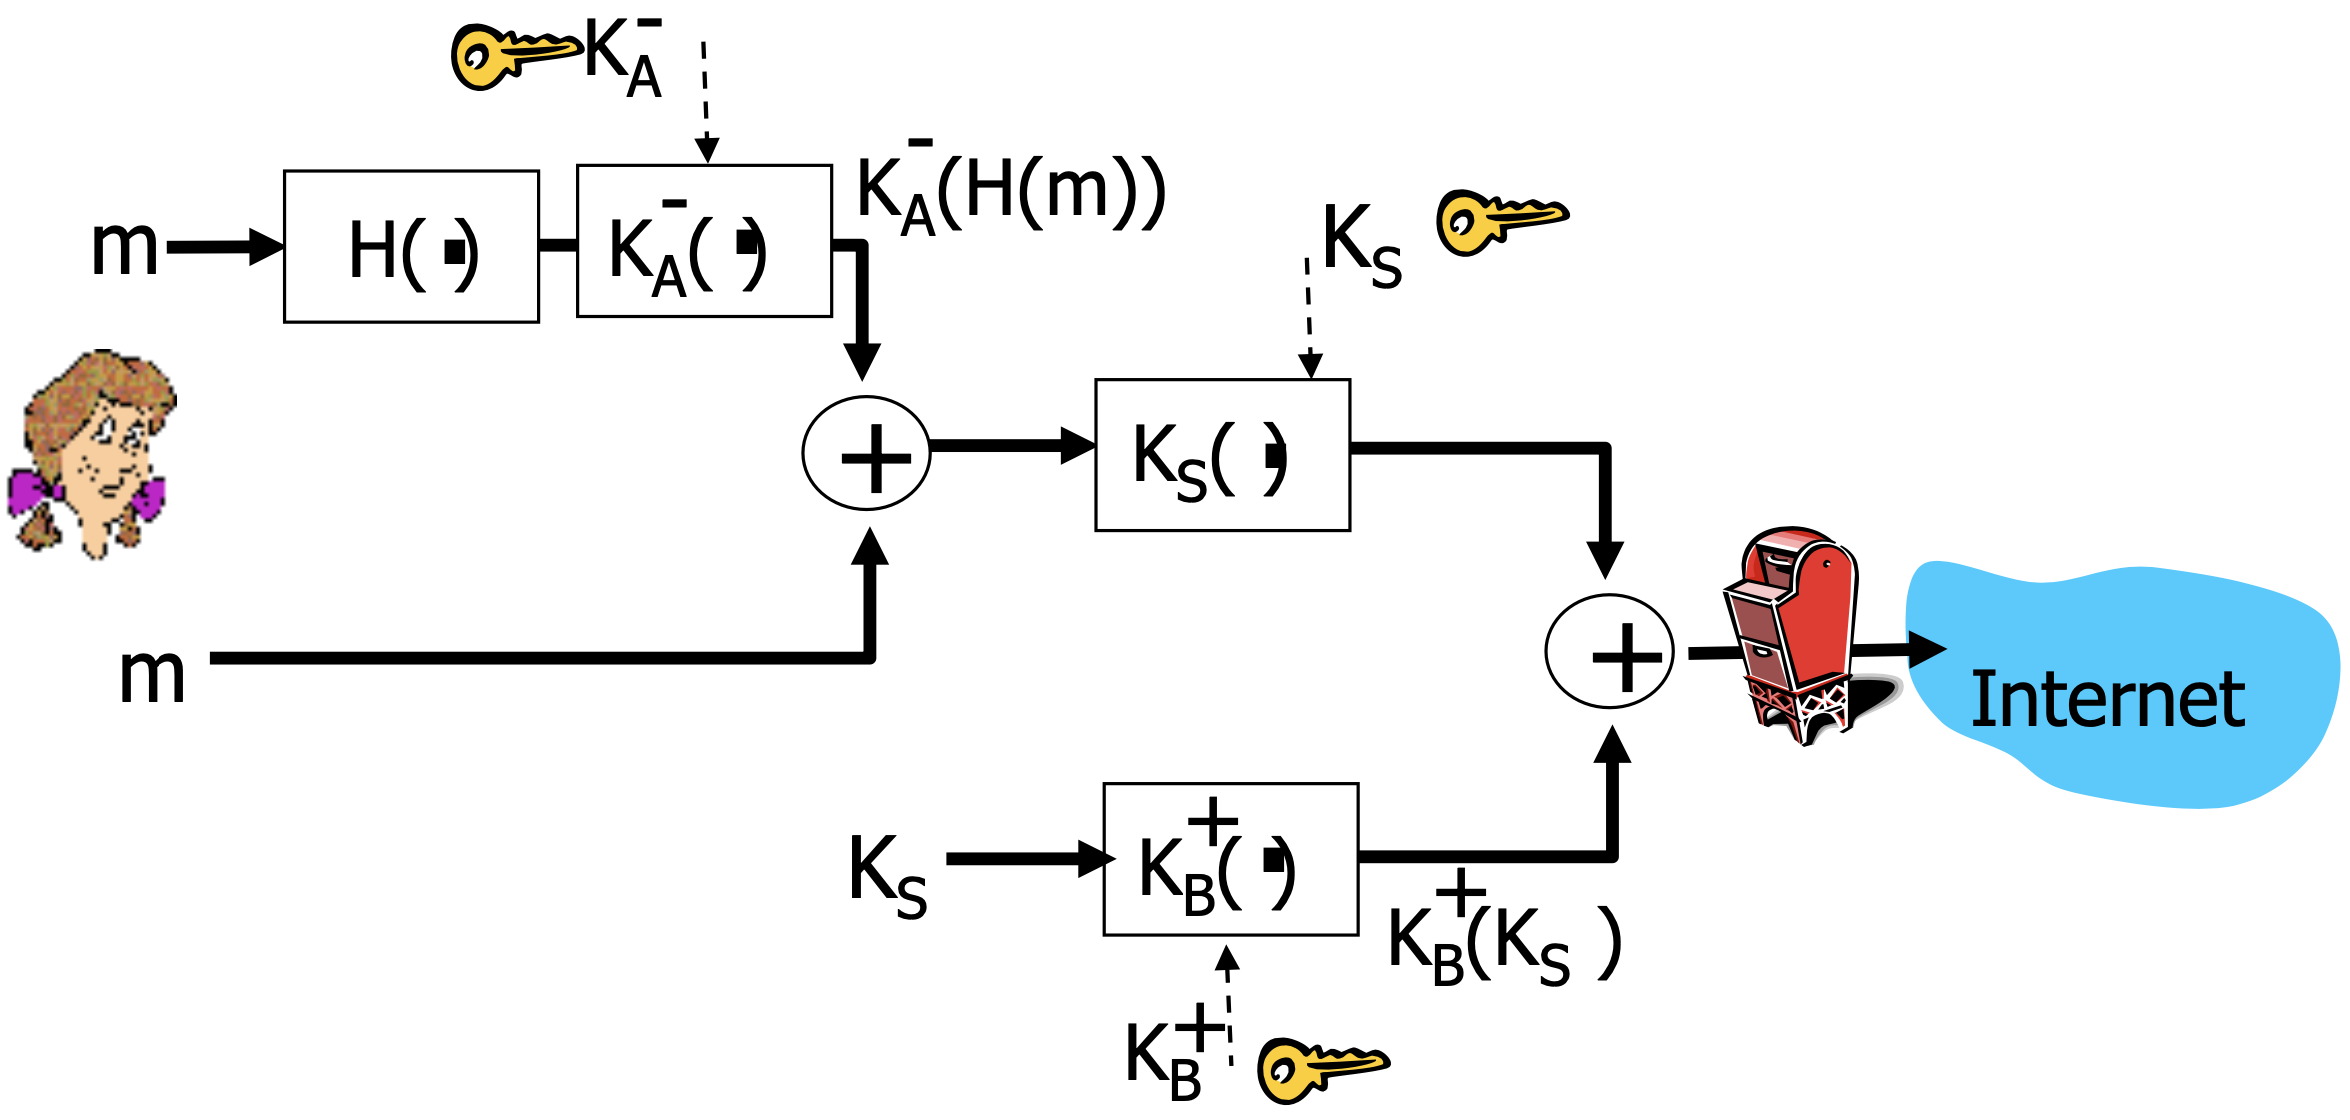
\includegraphics[scale=0.25]{Sicherheit_SMPT.png}
			\end{center}

	
	\subsection{Netzwerkmanagement}
							
			
			
			
			
